\documentclass[11pt]{article}

\usepackage[margin=1in]{geometry}
\usepackage{amsmath,amssymb}
\usepackage{booktabs}
\usepackage{graphicx}
\usepackage{microtype}
\usepackage[numbers,sort&compress]{natbib}
\usepackage[hidelinks]{hyperref}
\usepackage{enumitem}

\graphicspath{{figures/}}
\setlist{nosep}

\title{When Structure Is Not Utility: Localizing Failure Modes of Structural Interventions in Unsupervised Clustering}
\author{Anonymous Authors}
\date{}

\begin{document}
\maketitle

\begin{abstract}
Structural signals are widely used to shape unsupervised representations, but a
useful relation is not necessarily a useful intervention. We study this gap as
a mechanism-localization problem rather than as a search for another
architecture. The audited V1--V22 history contains 2,209 registry rows, 1,637
paired Delta ARI records, and 431 dataset/protocol/readout units; its 194
material-positive, 680 material-negative, and 763 observed-small rows form an
observational Failure Atlas. We then analyze a predeclared V21 case study with a
shared warmup branchpoint and budget-, donor-, eligible-set-, batch-, and
selection-noise-matched None, Random, and Topology policies. The primary
per-seed endpoint is
$S_{\mathrm{full\_ARI}}=\operatorname{ARI}_T-\operatorname{ARI}_R$; the reported
$S_d$ values are the dataset means of those three seed-level endpoints. The
confirmation means are $+0.044617$ for Baron Human and $-0.065332$ and
$-0.033410$ for Campbell and \texttt{hate\_speech}, respectively. Thus
topology-dependent selection has a conditional, sign-heterogeneous effect in
this audited case study, not universal superiority. Feature, gradient, and
local/global records remain diagnostics, not universal causal explanations. A
predeclared holdout produced zero of six evaluable panels; independent
validation is not established, and the status is recorded as
\texttt{inconclusive\_not\_completed}, not as a negative model result.
\end{abstract}

\section{Introduction}

Local neighborhoods, graphs, and related structural signals are established
ways to shape unsupervised representations \citep{xu2024sccdcg,li2025dcboost}.
They can provide useful inductive bias for sparse, high-dimensional observations,
but a structural signal is not itself a clustering objective. The operation that
selects a relation, applies a perturbation, updates a representation, and then
produces a partition can preserve, distort, or discard the information available
at the start.

We study the gap between \emph{structural opportunity} and
\emph{intervention utility}. A graph may contain a locally informative relation
while a learned selector chooses the wrong coordinates. A fixed-budget
intervention may damage cluster-defining features. An auxiliary objective may
compete with representation learning \citep{yan2026scmib}. Or a local geometric
improvement may fail to survive the global readout \citep{li2025dcboost}.
These stages are often collapsed into one score difference between a structural
variant and a baseline. Such a difference shows that a variant changed a score;
it does not identify whether the change came from the structural policy, the
generic intervention, the optimizer, or the readout.

The problem becomes sharper when evidence accumulates across exploratory
versions. Different versions may change preprocessing, intervention location,
training target, effective budget, stochastic schedules, or final readout.
Seeds and variants are then repeated measurements rather than independent data
sets. A credible synthesis must preserve protocol and dataset boundaries while
still exposing recurring patterns. It must also distinguish post-treatment
descriptors from pre-intervention properties and must not turn incomplete
computation into a negative result.

Our question is therefore: \textbf{why does apparently useful structural
information fail to translate reliably into unsupervised clustering utility?}
We use the localization chain

\begin{center}
\textbf{Opportunity $\rightarrow$ Selection $\rightarrow$ Intervention
$\rightarrow$ Representation $\rightarrow$ Readout}.
\end{center}

The chain asks whether an opportunity is measurable, whether topology changes
what is selected, whether a matched intervention is helpful, whether the
objective moves the representation compatibly, and whether local changes survive
the global readout. This is a study protocol and claim firewall, not a new
neural architecture.

\begin{figure}[t]
\centering
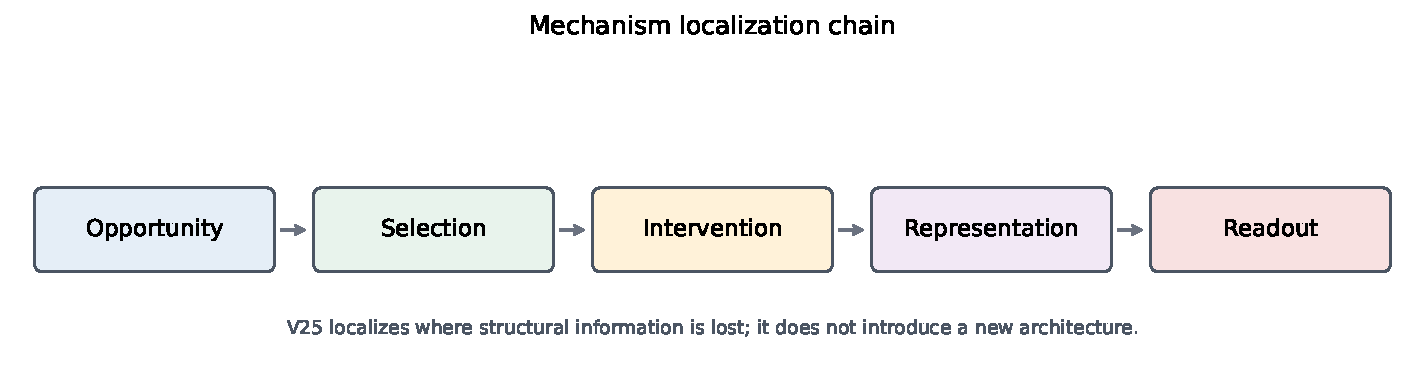
\includegraphics[width=0.98\linewidth]{V25_Figure2_mechanism_chain}
\caption{Frozen V25 mechanism-localization chain. The diagram is a protocol
schema for separating opportunity, policy, intervention, representation, and
readout; it is not a fitted architecture or a causal graph estimated from the
historical rows.}
\label{fig:chain}
\end{figure}

Our contributions are twofold. First, we provide an auditable observational
Failure Atlas for the V1--V22 history, with repeated-measurement units,
protocol/readout boundaries, and a separate V23/V24 boundary branch. Second, we
provide a matched V21 selection-policy decomposition that separates generic
intervention from topology-dependent selection and exposes conditional signs.
Feature, gradient, and local/global analyses localize possible failure stages;
they are not promoted to universal causal laws.

\section{Study Design and Methods}

\subsection{Evidence layers and statistical units}

The A0 registry records dataset, protocol, variant, seed, source and
preprocessing hashes, readout and $K$ provenance, structural source, selection
policy, intervention location, training target, measurement timing, causal
status, artifact availability, label/$K$ isolation, reuse provenance, and
alternative explanations. V1--V22 enter the quantitative atlas. V23 and V24
are registered as boundary evidence but are not pooled with
structural-intervention rows.

The primary retrospective unit is dataset/protocol/readout. Seed and variant
rows are repeated measurements. We do not treat the 1,637 paired records as
1,637 independent data sets. A1 uses raw Delta ARI as its primary descriptive
quantity; headroom-aware summaries and intervention-magnitude descriptors are
sensitivity or post-treatment diagnostics, not causal covariates.

The A1 numbers are imported historical metrics: A1 does not reload labels or
recompute historical ARI values. Consequently, the atlas preserves the
original evaluation and selection provenance, including the historical V21
dataset-selection bias, rather than presenting a newly harmonized label-free
benchmark.

\begin{table}[t]
\centering
\caption{Evidence layers and their inferential boundary.}
\label{tab:layers}
{\small
\setlength{\tabcolsep}{2pt}
\begin{tabular}{@{}p{0.13\linewidth}p{0.25\linewidth}p{0.22\linewidth}p{0.18\linewidth}@{}}
\toprule
Layer & Evidence & Statistical unit & Causal status \\
\midrule
A0/A1 & V1--V22 registry and atlas & dataset / protocol / readout & observational \\
A0 boundary & V23/V24 No-Go records & boundary record & isolated historical boundary \\
E1 & V21 matched N/R/T & dataset; seeds repeated & matched prospective case study \\
E2 & feature and optimizer diagnostics & dataset $\times$ seed & diagnostic/post-hoc \\
E3 & local/global replay boundary & artifact-complete case & observational boundary \\
Phase D & predeclared holdout & six panels & incomplete compute \\
\bottomrule
\end{tabular}
}

\end{table}

\subsection{Failure Atlas and mechanism triage}

A1 admits only artifact-complete cases to offline replay. Metadata-only
snapshots remain provenance records and cannot be reconstructed into replay
evidence. The atlas separates structural opportunity, baseline/headroom,
local/global conversion, and post-treatment magnitude descriptors. Because no
common fixed-graph/null opportunity endpoint exists across all historical
protocols, the atlas is observational rather than a pooled causal test of
structural quality.

A2 constructs a Claim--Evidence Matrix with historical support, counterexamples,
identifiability, required generality, fatal falsifiers, alternative
explanations, novelty, and required new compute. It can retain E1, cancel E1,
or authorize no prospective computation; it cannot invent an E4 after triage.
In the frozen artifacts A2 retained E1 and froze the selection claim, the
primary per-seed endpoint
$S_{\mathrm{full\_ARI}}=\operatorname{ARI}_T-\operatorname{ARI}_R$,
the claim-dependent holdout subset, and the practical threshold $\delta=0.03$.

\subsection{Matched V21 case study}

The prospective case study compares three arms:

\begin{align}
N&=\text{matched None},\\
R&=\text{matched Random assignment policy},\\
T&=\text{topology-dependent selection policy}.
\end{align}

The estimands are
\begin{align}
I_d &= Q(R)-Q(N),\\
S_d &= Q(T)-Q(R),\\
Q(T)-Q(N)&=I_d+S_d.
\end{align}

For E1, $Q$ is the clean-embedding, known-$K$ KMeans ARI for one seed. Thus
$S_{\mathrm{full\_ARI}}$ is the primary seed-level endpoint and
$S_d=\operatorname{mean}_{s\in\{42,123,7\}}S_{\mathrm{full\_ARI},d,s}$ is only
the dataset-level summary used for the four-state rule and figures. Pilot and
confirmation panels are audited and reported separately; they are not pooled.

The losses are frozen as
\begin{align}
L_N &= L_{\mathrm{scMAE}}+\lambda_iL_{\mathrm{InfoMax}},\\
L_R &= L_{\mathrm{scMAE}}+\lambda_iL_{\mathrm{InfoMax}}+\lambda_aL_{\mathrm{JS}}^R,\\
L_T &= L_{\mathrm{scMAE}}+\lambda_iL_{\mathrm{InfoMax}}+\lambda_aL_{\mathrm{JS}}^T.
\end{align}

All arms start from one branchpoint after warmup and Student-$t$ head
initialization and before the first assignment update. Base reconstruction
masks and donors, assignment donors, eligible coordinates, exact effective
budgets, batch order, topology statistics, Gumbel selection noise, and readout
randomness are shared or hash-audited. The Random arm uses zero topology logits
plus the same frozen Gumbel tensor; the Topology arm adds topology-dependent
logits. None preserves the reconstruction and InfoMax terms and optimizer state
but executes no assignment forward and no JS loss.

The primary readout is clean embedding plus known-$K$ KMeans. The Student-$t$
head is a secondary diagnostic. The full label vector is excluded from
preprocessing, graph construction, Gate, loss, optimizer updates, and all model
state transitions. Labels enter only after fitting for outer ARI/NMI evaluation;
benchmark-known $K$ may nevertheless be derived from the outer labels to size
the trainable head and primary readout. E1 is therefore a real-ground-truth,
known-$K$ benchmark, not fully label-free fitting.

The pilot contains cnae9, Mouse Retina, and SMS with seeds $[42,123,7]$; the
confirmation panel contains Baron Human, Campbell, and \texttt{hate\_speech}
with the same seeds. A dataset-level state is Positive or Negative only when
the mean effect exceeds $\pm0.03$ and at least two of three seed effects share
its sign. Observed-Small requires the mean and all three seed effects to be
smaller in absolute value; otherwise the state is Inconclusive. No three-seed
bootstrap is used to claim equivalence.

\subsection{Localization diagnostics}

E2-A compares topology-selected and eligible-but-not-selected coordinates, but
aggregates each metric at dataset-by-seed level. Coordinate-level distributions
are descriptive plots only. Fisher separation, mutual information, and
class-support enrichment are post-hoc label-aware descriptors and are not fit
inputs. E2-B records base, assignment, and InfoMax gradient geometry at T0, T1,
and T2. E2-C clones model, head, and Adam state and executes actual N/R/T Adam
one-step updates. These diagnostics do not establish a universal
objective-compatibility law.

E3 applies the artifact-complete replay gate and keeps label-free geometry
separate from post-hoc supervised neighborhood metrics. The frozen replay
summary has zero eligible rows (\texttt{candidate\_rows=0}), so no E3 replay
was run; the V23 local/global rows remain separate boundary evidence. A local
improvement accompanied by non-positive ARI is therefore only a possible
conversion-failure pattern, not a universal local-to-global theorem.

\subsection{Holdout and closure}

Before E1 outcomes, the holdout candidate pool, input adapters, normalization,
feature selection, graph/model inputs, source hashes, measurement schema, and
claim-dependent activation rule were frozen. The manifest records a scRNA
shortfall and does not silently fill it using outcomes. Phase C selected the
selection claim, so Phase D activated the N/R/T subset and primary
$S_{\mathrm{full\_ARI}}$ endpoint. The expected holdout contained six panels.
No panel produced an evaluable primary endpoint under the frozen dense decoder/
Adam resource path; this is incomplete compute, not an independent replication
result.

\section{Results}

\subsection{Historical Failure Atlas}

The registry contains 2,209 V1--V22 rows, including 1,637 paired Delta ARI rows
grouped into 431 dataset/protocol/readout units. The paired atlas contains 194
material-positive, 680 material-negative, and 763 observed-small rows at
$\delta=0.03$. The signs and magnitudes vary across intervention families and
protocols, but the registry does not provide one common structural-opportunity
endpoint. We therefore report these values as an observational atlas rather than
as a pooled causal estimate.

\begin{table}[t]
\centering
\caption{Counts in the frozen retrospective atlas. Rows are repeated records,
not independent data sets.}
\label{tab:atlas}
\begin{tabular}{lr}
\toprule
Quantity & Value \\
\midrule
V1--V22 registry rows & 2209 \\
Paired $\Delta$ARI rows & 1637 \\
Dataset/protocol/readout units & 431 \\
Material positive rows & 194 \\
Material negative rows & 680 \\
Observed-small rows & 763 \\
\bottomrule
\end{tabular}

\end{table}

\begin{figure}[t]
\centering
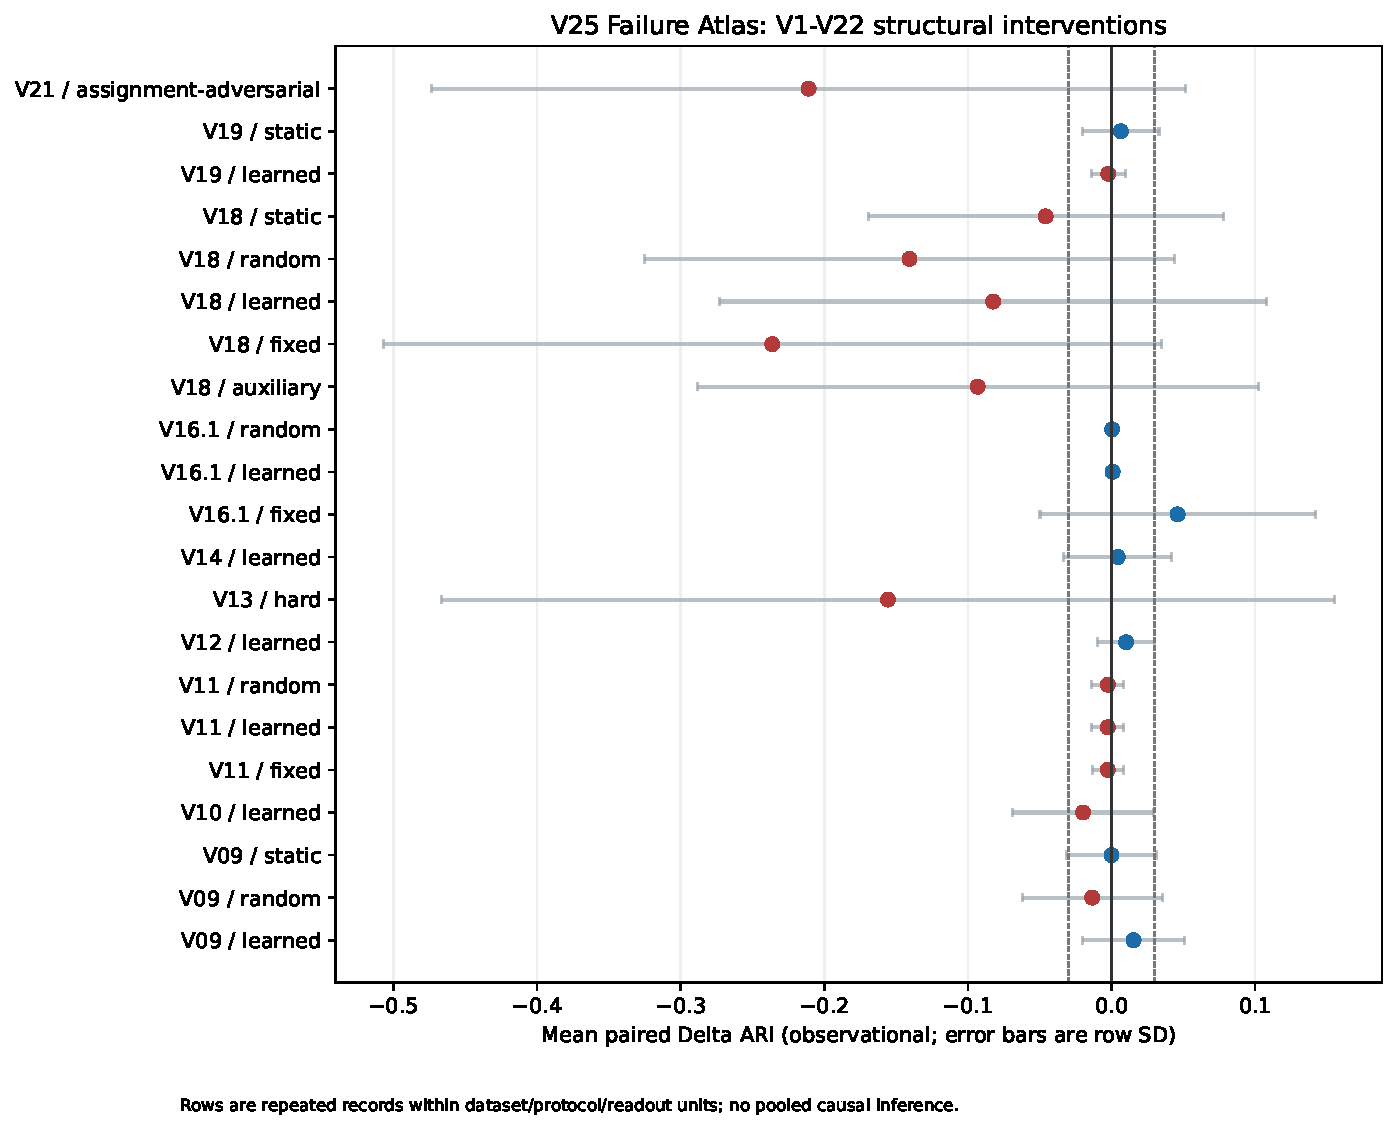
\includegraphics[width=0.98\linewidth]{V25_Figure1_failure_atlas}
\caption{V1--V22 Failure Atlas. The display is observational and stratified by
version/family; it is not a pooled causal estimate.}
\label{fig:atlas}
\end{figure}

\subsection{Matched selection effects}

The audited E1 panels pass the full matching and label-isolation contract. The
per-seed primary endpoint is $S_{\mathrm{full\_ARI}}$; the confirmation dataset
means $S_d=\operatorname{mean}_s(S_{\mathrm{full\_ARI}})$ are shown in
Table~\ref{tab:e1} and Figure~\ref{fig:e1}.
The primary selection effect changes sign across the three confirmation data
sets. The generic intervention effect is also heterogeneous: it is positive for
Campbell, observed-small for \texttt{hate\_speech}, and inconclusive for Baron
Human. This decomposition separates generic intervention from the topology
policy increment; it does not prove either component universal.

\begin{table}[t]
\centering
\caption{Confirmation means for the matched V21 decomposition. Each row is a
dataset mean over three repeated seeds.}
\label{tab:e1}
\begin{tabular}{lrrl}
\toprule
Dataset & $I_d$ & $S_d$ & $S_d$ state \\
\midrule
Baron Human & -0.011463 & +0.044617 & Positive \\
Campbell & +0.132841 & -0.065332 & Negative \\
hate\_speech & -0.002671 & -0.033410 & Negative \\
\bottomrule
\end{tabular}

\end{table}

\begin{figure}[t]
\centering
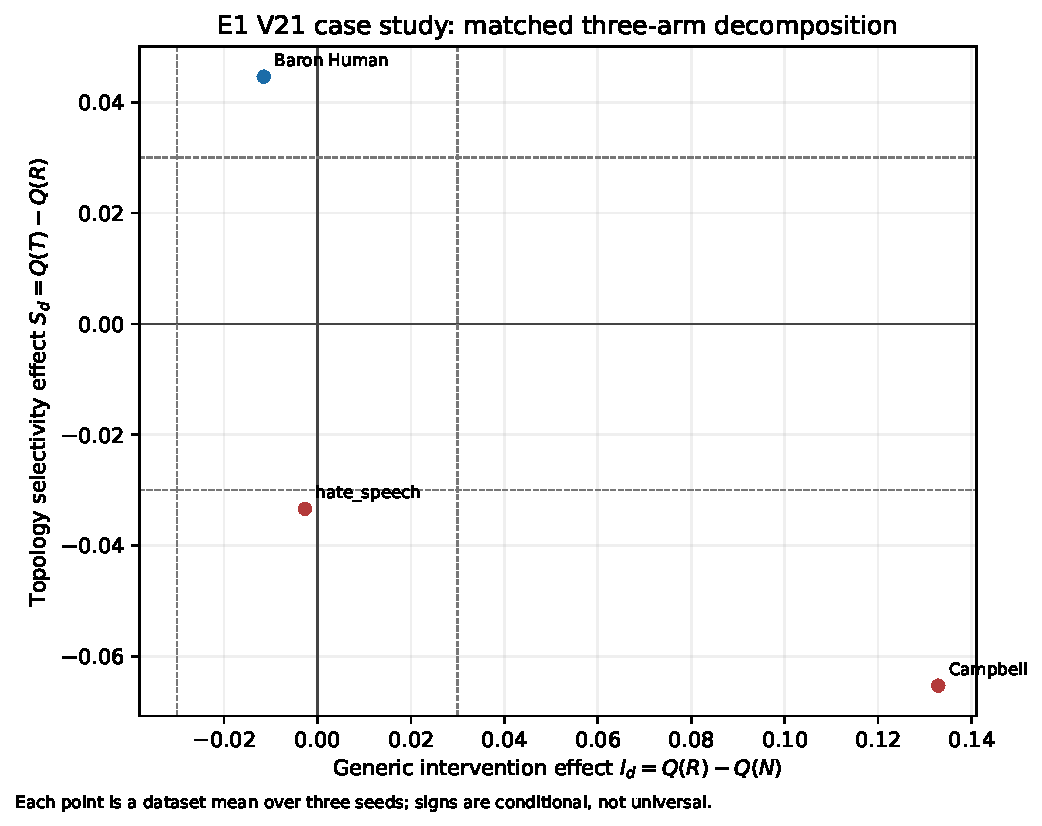
\includegraphics[width=0.78\linewidth]{V25_Figure3_e1_selectivity}
\caption{Generic intervention effect $I_d$ versus topology selectivity effect
$S_d$. The signs are conditional case-study evidence, not a population claim.}
\label{fig:e1}
\end{figure}

The pilot gate passed because at least two of three pilot datasets showed a
seed-stable material effect in either $I_d$ or $S_d$; signs were not required to
agree. Pilot and confirmation are not pooled: the confirmation panel alone
supplies the three case-study values above. The result is therefore evidence for
conditional utility and heterogeneity, not a reason to search for a universally
beneficial selector.

\subsection{Localization diagnostics}

E2 produces dataset-by-seed semantic summaries and gradient/one-step records
under the frozen N/R/T protocol. These artifacts permit inspection of selected
feature semantics and optimizer-direction changes, but they do not produce a
stable cross-dataset objective-conflict rule. Figure~\ref{fig:diagnostics}
shows the diagnostic geometry without fitting a cross-dataset causal model.

\begin{figure}[t]
\centering
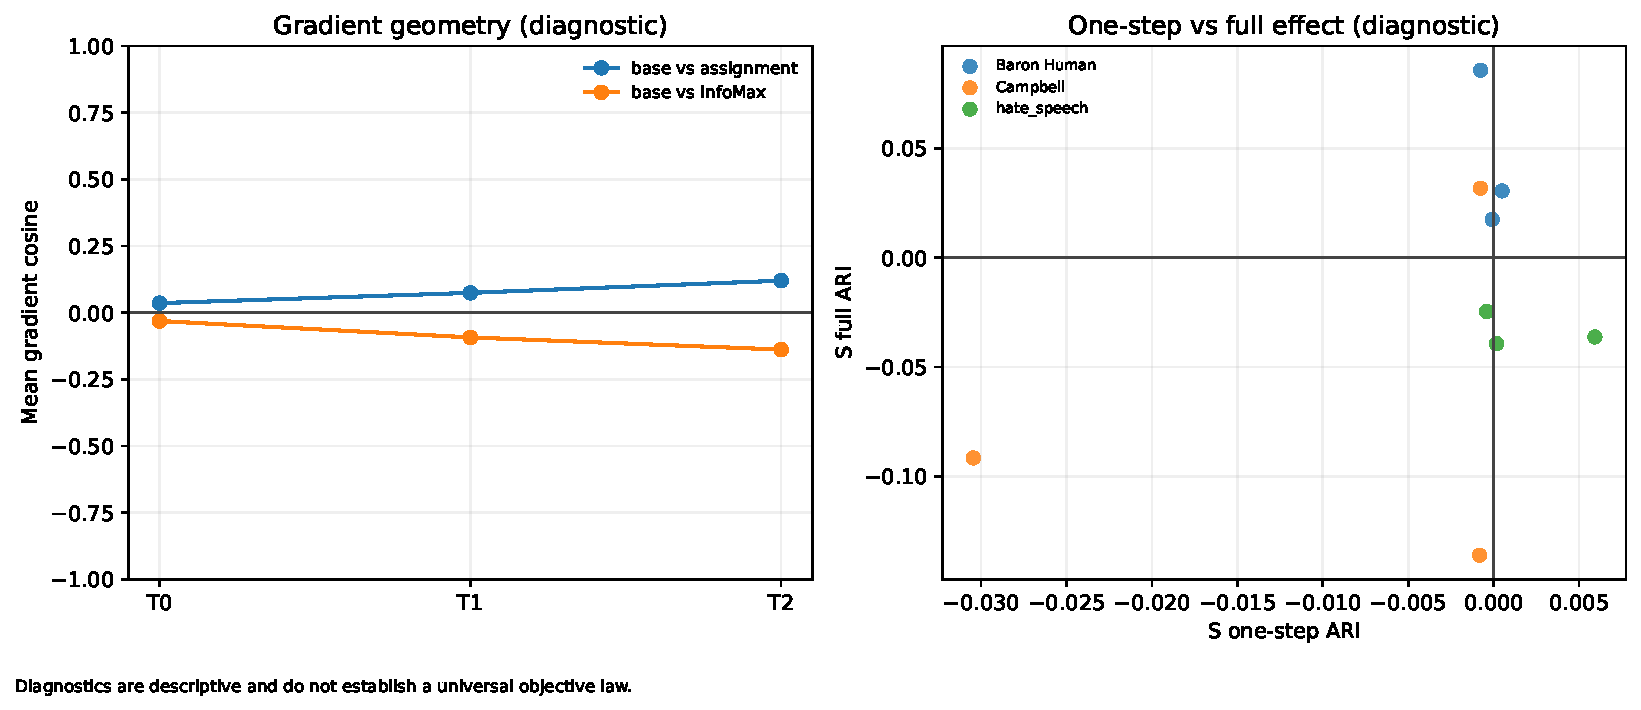
\includegraphics[width=0.98\linewidth]{V25_Figure4_diagnostics}
\caption{E2 diagnostic geometry. Gradient cosines and one-step/full effects are
descriptive records; they are not a universal objective-compatibility law.}
\label{fig:diagnostics}
\end{figure}

The E3 replay gate found zero artifact-complete candidate rows, so no replay was
run. The separate V23 boundary rows are retained only to show why local and
global readouts must be measured separately; they do not support a universal
conversion law.

\begin{figure}[t]
\centering
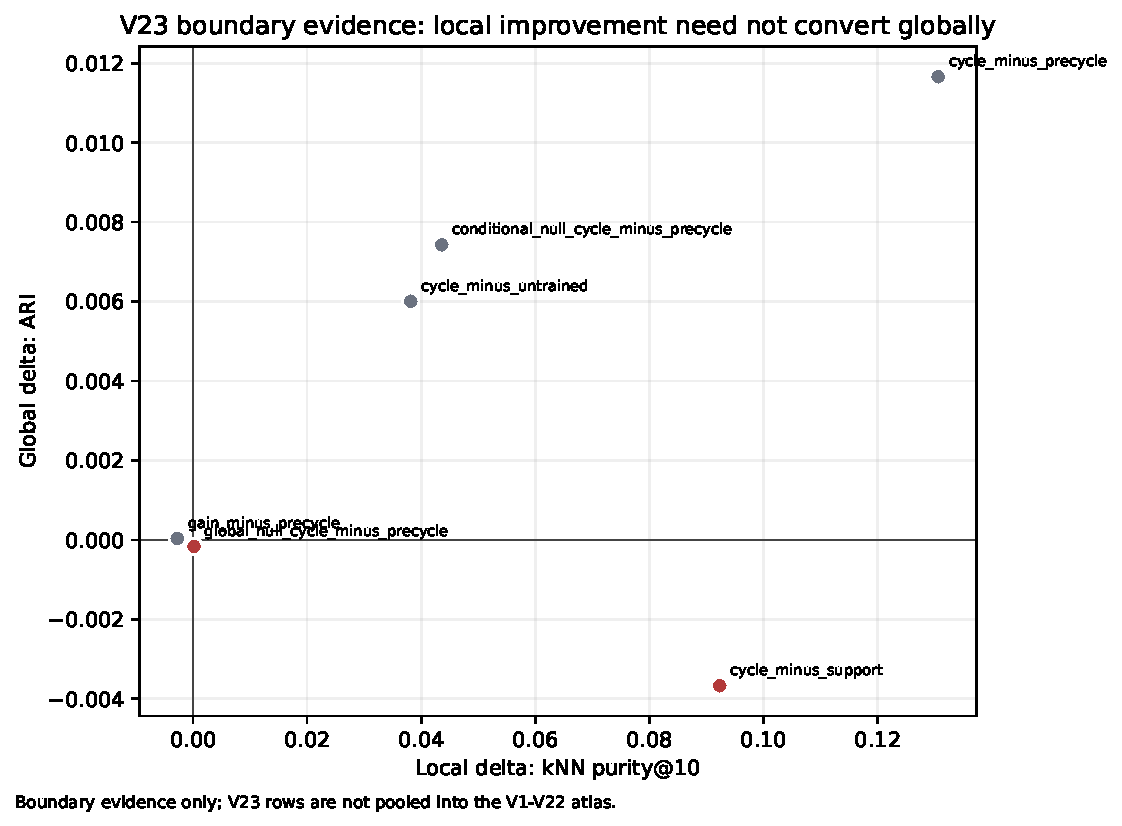
\includegraphics[width=0.78\linewidth]{V25_Figure5_local_global_boundary}
\caption{V23 local/global boundary evidence. These rows are kept outside the
V1--V22 atlas and are not a universal theorem.}
\label{fig:boundary}
\end{figure}

\subsection{Independent validation status}

The holdout has no evaluable endpoint: zero of six panels completed under the
frozen protocol, and the recorded cause is the dense decoder/Adam resource
boundary. Independent validation is therefore not established. We do not use
this incomplete compute to falsify the selection claim or report a negative
performance result.

\section{Discussion}

The central result is a separation between structural opportunity and structural
intervention effect. In the broad history, heterogeneous signs appear across
protocols and readouts, but the historical data cannot identify one common
opportunity treatment. In the narrower V21 counterfactual, topology-dependent
selection still changes sign after generic intervention and selection noise are
matched. The defensible conclusion is a conditional, sign-heterogeneous
selection effect: how and where structure intervenes matters at least as much
as whether a structural signal can be measured.

This result changes what a next method would need to demonstrate. A more
elaborate selector is not justified merely because a previous selector failed.
A convincing method would need to show, under a matched generic-intervention
control, that its policy changes the primary readout in a stable direction. It
would also need to separate label-free training evidence from post-hoc semantic
diagnostics. The current study does not propose that method; it supplies the
failure-localization protocol needed before designing one.

The findings also explain why local geometry, reconstruction difficulty, and
assignment stability should not be used interchangeably. A local metric can be
post-treatment and label-aware \citep{li2025dcboost}, a reconstruction loss can
reward a difficult coordinate without improving the partition
\citep{yan2026scmib}, and a training head can disagree with a clean-embedding
KMeans readout. Treating these as the same utility signal would recreate the
experimental loop this study is designed to stop \citep{li2025lfss}.

\section{Limitations and Conclusion}

First, the historical atlas has no common structural-opportunity endpoint. Its
value is breadth and failure coverage, not causal identification across all
versions; A1 imports historical metrics and retains the historical V21
dataset-selection bias. Second, the prospective evidence is a six-dataset V21
case study with known-$K$ evaluation; its conditional signs cannot be generalized
to every structural intervention or domain. Third, E2 and E3 are diagnostics,
with dataset-by-seed aggregation and post-hoc label-aware descriptors; E3 had no
eligible replay rows, and neither stage proves objective conflict, readout
failure, or a universal local-to-global law. Fourth, the independent holdout is
zero of six and \texttt{inconclusive\_not\_completed}, so independent validation
remains unestablished; the frozen candidate/adapter manifest and its pool
shortfall were fixed before outcomes, while the recorded CUDA failure is only
incomplete compute. Finally, A2 retained E1 but prohibited E4, new Gates/losses,
and V26 or rescue routes; no new architecture or comparison was used to make the
narrative more attractive.

\paragraph{Conclusion.}
Structural information is not synonymous with clustering utility. The audited
history provides an observational atlas of heterogeneous intervention outcomes,
and a matched V21 case study shows that topology-dependent selection can be
positive or negative across data sets even when generic intervention and
selection noise are controlled. The defensible contribution is therefore not
another Gate; it is a mechanism-localization and claim-firewall protocol that
identifies where structural information may be lost and states clearly what the
current evidence does not establish.


\appendix
\section{Evidence and audit boundary}
The paper-facing bundle is an analysis-only export from frozen V25 artifacts.
It does not retrain a model or treat rows, seeds, or coordinates as independent
population units. The exact source files and SHA256 values used to generate the
tables are recorded in
\texttt{tables/latex\_assets\_manifest.json}. The full per-job contract,
branchpoint, schedule, label-isolation, and incomplete-compute records remain in
\texttt{result/V25\_systematic\_mechanism\_study/}.

The scMAE source is not cited because its local PDF has not passed the repository
citation lifecycle. This is an explicit provenance boundary, not a substituted
reference. The paper also does not report any independent holdout result: the
frozen holdout status is \texttt{inconclusive\_not\_completed}.

\bibliographystyle{plainnat}
\bibliography{references}

\end{document}
